% \chapter{Vorbereitung und Konfiguration der Simulationskette}
% \chapter{Simulation eines Detektors in verschiedenen Wassertiefen}
\chapter{Simulation eines Detektors unter verschiedenen Wassertiefen}

%Einleitung was hier passiert

Aufgrund der Bergbauvergangenheit sind im Ruhrgebiet viele Bohrungen gemacht worden.
In einige der Bohrungen ist ein Metallrohr mit einem Durchmesser von \SI[]{10}[]{m} 
eingelassen.
Um den Wasserstand der trocken gelegten Schichten zu überwachen
ist die Idee dieser Arbeit in eines dieser Rohre einen zylinderförmigen Detektor 
herunterzulassen und zu ermitteln welche Detektorraten erwartet werden.

Um zu ermitteln in welchen Rahmen der Wasserstand dieser Schichten messbar ist,
wird für den zylinderförmiger Detektor eine Grundfläche von 
\SI[]{75}[]{cm^2} angenommen. Er soll sich auf dem Boden der Bohrung befinden.
Es wird anhand des Schichtverzeichnisses der Bohrung ein Bodenmodell erstellt,
welches die unterschiedlichen Bodenzusammensetzungen über Variationen der
\textit{Standardrock}-Dichte.
Dieses ist die Basis für die Propagation mit PROPOSAL.
Kosmische Myonen werden mithilfe einer Parametrisierung des Myonenflusses auf Meereshöhe
mit EcoMug erzeugt.

% todospäter
% \marktodo{veranschaulichung des messaufbaus: Luft, Boden, Wasser Detektor???} 

% Die Simulation besteht im Wesentlichen aus zwei Teilen. 
% Als Erstes werden Myonen aus einer Parametrisierung 
% des Myonenflusses auf Meereshöhe mit EcoMug gezogen und zwischengespeichert.
% Diese Myonen werden dann von PP durch das Bodenmodell bis zu dem Detektor propagiert. 
% Als Ergebnis liefert PROPOSAL, wie viele Myonen am Detektor angekommen sind.
% Die entsprechende Detekorzählrate wird im Kapitel Ergebnisse errechnet.




\section{Bodenmodell}
\label{sec:bodenmodell}
%%%%%%%%%%%%%%%%%%%%%%%%%%%%%%%%%%%%%%%%%%%%%%%%%%%%%%%%%%
% bohrung eckdaten, grundlage
%%%%%%%%%%%%%%%%%%%%%%%%%%%%%%%%%%%%%%%%%%%%%%%%%%%%%%%%%%
\subsection{Beschreibung der Bohrung}
Als Basis für das Bodenmodell dient eine Bohrung in der 
Kirchheller Heide\footnote{
    \url{boreholemap.bgr.de/mapapps/resources/apps/boreholemap/} 
    Standort: (351221,19 5719599,6) 
    ID: DABO\_65808 nahe dem Schwarze Heide Airport},
welches freundlicherweise von 
Prof. Dr. Ing. Tobias Rudolph\footnote{Technische Hochschule Georg Agricola - Forschungszentrum Nachbergbau}
zur Verfügung gestellt wurde.
In Abb. \ref{fig:Schichtverzeichnis_auszug} ist ein Ausschnitt des Schichtverzeichnis der Bohrung zu sehen.
Das vollständige Schichtverzeichnis befindet sich im Anhang
\ref{fig:Schichtverzeichnis_komplett}

\begin{figure}[h]
    \centering
    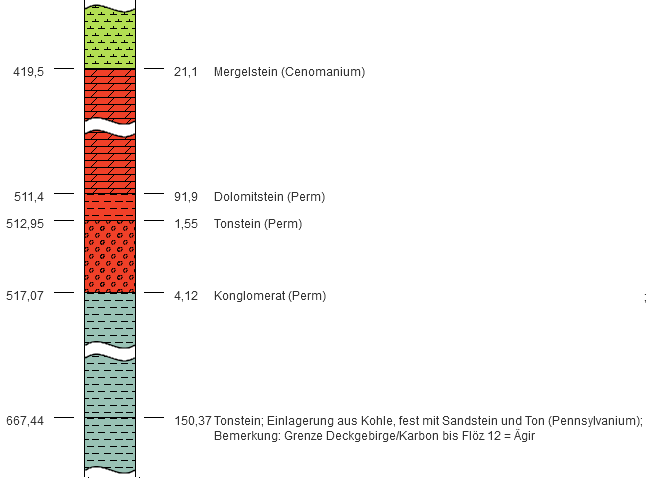
\includegraphics[width=0.97\textwidth]{schichtverzeichnis_auszug.png}
    \caption{Ein Auszug aus einer Bohrung in der Kirchheller Heide 
    Die Tiefe in Metern (links) ist als das untere Ende der Schicht gemeint,
    d.h. die Dolomit-Schicht geht von 419,5 bis 511 Metern.
    Die rechte Zahl ist die Höhe der Schicht in Metern.
    Hinter der Bodenart ist die jeweilige erdgeschichtliche Epoche in Klammern.
    Das vollständige Verzeichnis ist im Anhang \ref{sec:alle_schichten} zu sehen.}
    \label{fig:Schichtverzeichnis_auszug}
\end{figure}
 
Die Schichten von \num{1259} bis \SI{419,5}{m} (siehe Abb. \ref{fig:Schichtverzeichnis_auszug})
wurden aufgrund des Bergbaus in der Region trocken gelegt und während der Benutzung trocken gehalten 
(im folgenden \textit{Wasser-Schichten genannt}).
Jene Schichten haben ein sog. Hohlraumvolumen von ca. \num{5} bis \SI{15}{\percent}
welche naturgemäß mit Wasser gefüllt sind.
Das Hohlraumvolumen entspricht im Allgemeinen dem das, was von Kristallen 
in einer dichtesten Kugelpackung erwartet wird.
Zusätzlich zu dem Hohlraumvolumen müssen Risse berücksichtigt werden, welche zusätzlich 
\num{5} bis \SI{10}{\%} an Volumen ausmachen können und sich ebenfalls mit Wasser
füllen können.

Die Geschwindigkeit des Wasseranstiegs liegt in Größenordnungen von 
\SI{10}{cm} pro Woche. 

%%%%%%%%%%%%%%%%%%%%%%%%%%%%%%%%%%%%%%%%%%%%%%%%%%%%%%%%%%
%  modell erstellen
%%%%%%%%%%%%%%%%%%%%%%%%%%%%%%%%%%%%%%%%%%%%%%%%%%%%%%%%%%
\subsection{Umsetzung des Bodenmodells}
% Ziel ist es bei verschiedenen Wasserständen innerhalb der 
% entsprechenden Schichten die Detektorrate zu simulieren.
Es wird nun ein Bodenmodell anhand der Bohrung erstellt.

Zunächst wird festgestellt, dass die einzelnen Schichten jeweils aus einer 
Zusammensetzung verschiedener Gesteinsarten bestehen.
Da in PROPOSAL nicht die Möglichkeit besteht beliebige Gesteine
in ihrer chemischen Zusammensetzung zu modellieren, werden die Schichten mit 
dem Medium 
\textit{Standardrock}\footnote{Mit \textit{Standardrock} ist ein Material mit $Z = 11$, $A = 22$ und einer Dichte
von $\rho = \SI{2.65}[]{g/cm^3}$ gemeint \cite{Chirkin2015}.}
genähert.
Die Dichten werden entsprechend der echten Medien gesetzt.
Als Dichte der Schichten wird der Mittelwert zwischen $\rho_\mathrm{min}$
und $\rho_\mathrm{max}$ der jeweiligen 
Gesteinsarten\footnote{
    Tonstein, Dolomitstein, Sandstein: \cite{JS},
    Kalkstein \cite{RC},
    Mergelstein \cite{VNK},
    Sand \url{hausjournal.net/dichte-sand}}
benutzt (siehe Tabelle \ref{tab:gesteinarten})
In Abb. \ref{fig:dichte_modell} ist das Bodenmodell als Plot gegen die Tiefe abgebildet.

\begin{table}[h]
    \caption{Benutzte Dichten der verschiedenen Gesteinsarten in [\si[]{g/cm^3}].
    KS steht für Kalkstein, TS für Tonstein.}
    \centering\begin{tabular}{c c c c}
        Gesteinsart & $\rho_\mathrm{min}$ & $\rho_\mathrm{max} $ & $\rho_\mathrm{avg}$ \\
        \toprule
        Sand & 1,43 & 1,47&1,45 \\
        Tonmergelstein (\SI[]{20}[]{\%} KS, \SI[]{80}[]{\%} TS)&&&1,87 \\
        Kalkmergelstein (\SI[]{70}[]{\%} KS, \SI[]{30}[]{\%} TS)&&&2,045 \\
        Kalkstein  & 1,55 & 2,75 & 2,15 \\
        Mergelstein & 1,2 & 3 & 2,1 \\
        Dolomitstein & 2,4 & 2,9 & 2,65 \\
        Tonstein & 1,3 & 2,3 & 1,8 \\
        Sandstein & 2 & 2,8 & 2,4 \\
        % Konglomerat\footnote{\url{steine-und-minerale.de/atlas.php?f=3&l=K&name=Konglomerat}} & 2,3 & 2,6 & 2,45 \\
    \end{tabular}
    \label{tab:gesteinarten}
\end{table} 

%  \marktodo{rausgeschmissen sinnvoll?} 
% Des Weiteren sind einige Schichten unter
% \SI[]{1}[]{m}  \marktodo{wo mache ich die grenze?}
% Da so kleine Schichten im Anbetracht der bereits gemachten Näherungen
% keinen Mehrwert an Genauigkeit liefern, werden jene ignoriert.
% Die freie Lücke wird mit der darüber liegenden Schicht aufgefüllt.

\begin{figure}[h]
    \centering
    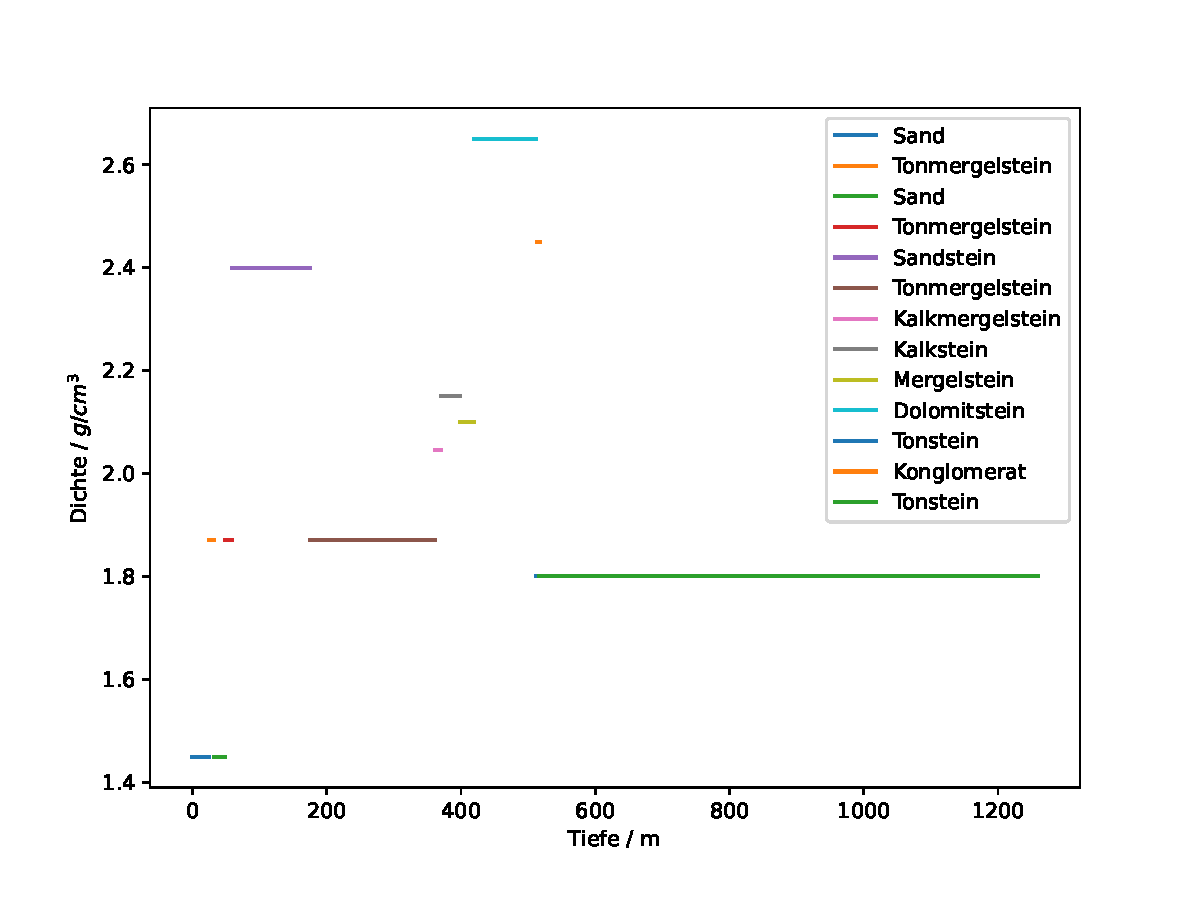
\includegraphics[width=\textwidth]{geology_modell_full.pdf}
    \caption{Das Bodenmodell nach Dichte und Tiefe aufgelöst.
    Der Tonstein in grün rechts, 
    sowie die Dolomitschicht oben in hellblau, können mit Wasser vollaufen.}
    \label{fig:dichte_modell}
\end{figure}

% wie wird volllaufen mit wasser modelliert.
Zur Modellierung der Wasser-Schichten,
wird angenommen, dass die Dichte 
einer Wasser-Schicht, das Gestein mit einem
Hohlraumvolumen von \SI[]{10}[]{\%} repräsentiert. 
Es wird also für Wasser-Schichten $\rho_\mathrm{Gestein10\%} == \rho_\mathrm{avg}$ angenommen.
Im trockenem Zustand wird der Hohlraum mit einer Luftdichte von 
$\rho_\mathrm{Luft} = \SI[]{0}[]{g/cm^3}$ genähert.
Daraus folgt 
\begin{equation}
    \rho_\mathrm{Gestein0\%} = \rho_\mathrm{Gestein10\%} / \num[]{0,9}.
\end{equation}
Mit $\rho_\mathrm{Gestein0\%}$ als die Dichte des Gesteins ohne Hohlraumvolumen.
Wenn ein Gestein mit Wasser vollläuft, wird die neue Dichte $\rho_\mathrm{nass}$ über
\begin{equation}
    \rho_\mathrm{nass} = 0,9*\rho_\mathrm{Gestein0\%} + 0,1*\rho_\mathrm{Wasser}
\end{equation}
berechnet. Für die Dichte des Wasser $\rho_\mathrm{Wasser}$ wird 
$\SI[]{1.0}[]{g/cm^3}$ \cite{Patterson_1994} angenommen.

Für die Tonstein-Schichten bspw. mit $\rho = \SI[]{1,8}[]{g/cm^3}$ 
steigt die Gesamtdichte mit Wasser auf \SI[]{1,9}[]{g/cm^3}.
Also eine effektive Erhöhung um ca. \SI[]{5,5}[]{\%}.



% \section{Konfiguration von EcoMug}
\section{Myonenfluss}
\label{sec:myonenfluss}
%%%%%%%%%%%%%%%%%%%%%%%%%%%%%%%%%%%%%%%%%%%%%%%%%
% gaisser param
%%%%%%%%%%%%%%%%%%%%%%%%%%%%%%%%%%%%%%%%%%%%%%%%%

Zur Beschreibung des Myonenflusses auf der Erde wird die 
\textit{Gaisser}-Parametrisierung \cite{Alexandrov2017} verwendet:
\begin{equation}
        \frac{\mathrm{d}N_{\mu}}{\mathrm{d}E_{\mu}\mathrm{d}\Omega} \approx \frac{0.14 E_{\mu}^{-2.7}}{\text{GeV cm$^2$ s sr}} \left(\frac{1}{1+1.1 E_{\mu}\cos \theta / (115 \text{GeV})} 
        + \frac{0.054}{1+1.1 E_{\mu}\cos \theta / (850 \text{GeV})}\right).
    \label{eqn:dN_dE}
\end{equation}

% \begin{equation}
    %     \begin{split}
        %     \frac{\mathrm{d}N_{\mu}}{\mathrm{d}E_{\mu}\mathrm{d}\Omega} &\approx \frac{0.14 E_{\mu}^{-2.7}}{\text{GeV cm$^2$ s sr}} \left(\frac{1}{1+1.1 E_{\mu}\cos \theta / (115 \text{GeV})} \\\
        %      &+ \frac{0.054}{1+1.1 E_{\mu}\cos \theta / (850 \text{GeV})}\right)
        %     \end{split} 
        % \end{equation}
        
        % \begin{multline}
%     d^2 = a^2 + b^2 + c^2 \geq a^2 + b^2 = a^2 + b^2 + 2ab - 2ab = (a+b)^2 - 2ab \\\ \geq -2ab
% \end{multline} 

% \begin{multline}
%     \frac{\mathrm{d}N_{\mu}}{\mathrm{d}E_{\mu}\mathrm{d}\Omega} \approx \frac{0.14 E_{\mu}^{-2.7}}{\text{GeV cm$^2$ s sr}} \left(\frac{1}{1+1.1 E_{\mu}\cos \theta / (115 \text{GeV})} \\\ + \frac{0.054}{1+1.1 E_{\mu}\cos \theta / (850 \text{GeV})}\right)
% \end{multline} 
    
% \label{eqn:dN_dE}
$N_{\mu}$ ist die Anzahl an Myonen, $E_{\mu}$ die Myonen Energie 
und $\Omega$ der Raumwinkel. Die Parametrisierung modelliert den Myonenfluss auf Meereshöhe.

Die zwei Terme in Klammern repräsentieren
jeweils die Beiträge über Zerfälle von Pionen bzw. Kaonen, wie beschrieben in Kap. \ref{sec:theorie}.
Die Parametrisierung gilt unter zwei Annahmen. Es wird die Krümmung der Erde vernachlässigt, 
welche den Zenit-Winkel einschränkt. Des Weiteren wird der Myon Zerfall vernachlässigt.
Folgende Einschränkungen gelten:
\begin{align}
    \theta < 70° \;\; \mathrm{und} \;\; E_\mu > \frac{\SI[]{100}[]{GeV}}{\cos \theta}.
\end{align}
Zur Vereinfachung wird angenommen dass das Bohrloch auf Meereshöhe beginnt. 
%  \marktodo{im EcoMug paper nachgucken welche einschränkungen deren parametrisierung hat} 
% Die Myo
% Die ursprüngliche Energien der Myonen die am Detektor ankommen im Kontext dieser Arbeit,
% liegen weit über $\SI[]{100}[]{GeV}$ daher ist die zweite Bedingung auch erfüllt.

Zur Einhaltung dieser wird in EcoMug das Maximum für den Winkel $\theta$ auf $30°$ konfiguriert.
Da die Myonen mehr als \SI[]{600}[]{GeV} benötigen um den Detektor zu erreichen,
ist die Zweite Bedingung auch erfüllt.
Es wird für die Erzeugung der Myonen mit EcoMug der Energiebereich von \SI[]{600}[]{GeV} bis 
\SI[]{200}[]{TeV} gewählt.
In Abb. \ref{fig:ecomugplot} ist das verwendete Energiespektrum aus EcoMug zu sehen.

\begin{figure}[]
    \centering
    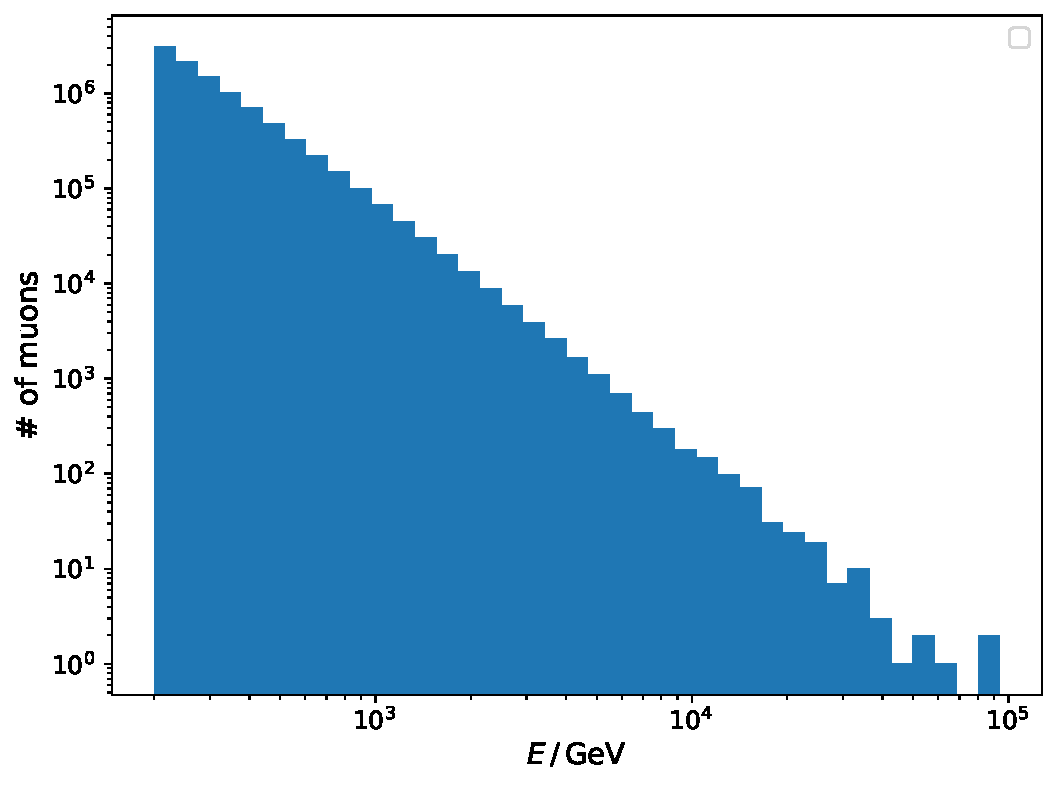
\includegraphics[width=0.7\textwidth]{Ecomug_spektrum779.pdf}
    \caption{Das verwendete Energiespektrum, mit EcoMug erzeugt.}
    \label{fig:ecomugplot}
\end{figure}


% \marktodo{ ecomug plots:
% energieverteilung mit cut
% winkelverteilung}

Zur Übertragung der Simulationsdaten auf die echte Welt, wird die 
Myonenfluss-Parametrisierung \eqref{eqn:dN_dE} über 
$E$ in den Grenzen \SI[]{600}[]{GeV} bis \SI[]{200}[]{TeV}, sowie
$\Omega$ von $0°$ bis $30°$ integriert.
Bei einer angenommenen Detektorgrundfläche von 
\SI[]{75}[]{cm^2} ergibt sich eine Myonenrate von:
\begin{align}
    \Phi_0 = 1.0857\:  \frac{\mathrm{Myonen}}{\mathrm{Tag}}.
\end{align}

Zur Berechnung der Detektorrate in Abhängigkeit zur Tiefe wird gerechnet:
\begin{equation}
    \Phi_h = \Phi_0 * a 
\end{equation}
$\Phi_h$ als Detektorrate mit dem Wasserstand $h$ und $a$ 
als der Anteil der Myonen, die es zum Detektor geschafft haben. 

Es wird angenommen, das der Detektor jedes Myon, das ihn trifft, messen kann.
Eine Detektion über die seitliches Flächen des Detektors wird nicht berücksichtigt.
Im Gegensatz zur echten Welt wird keine langsam steigende Wasserhöhe simuliert,
sondern die Messrate mehrerer statischen Wasserstände.

\begin{figure}[h]
    \centering
    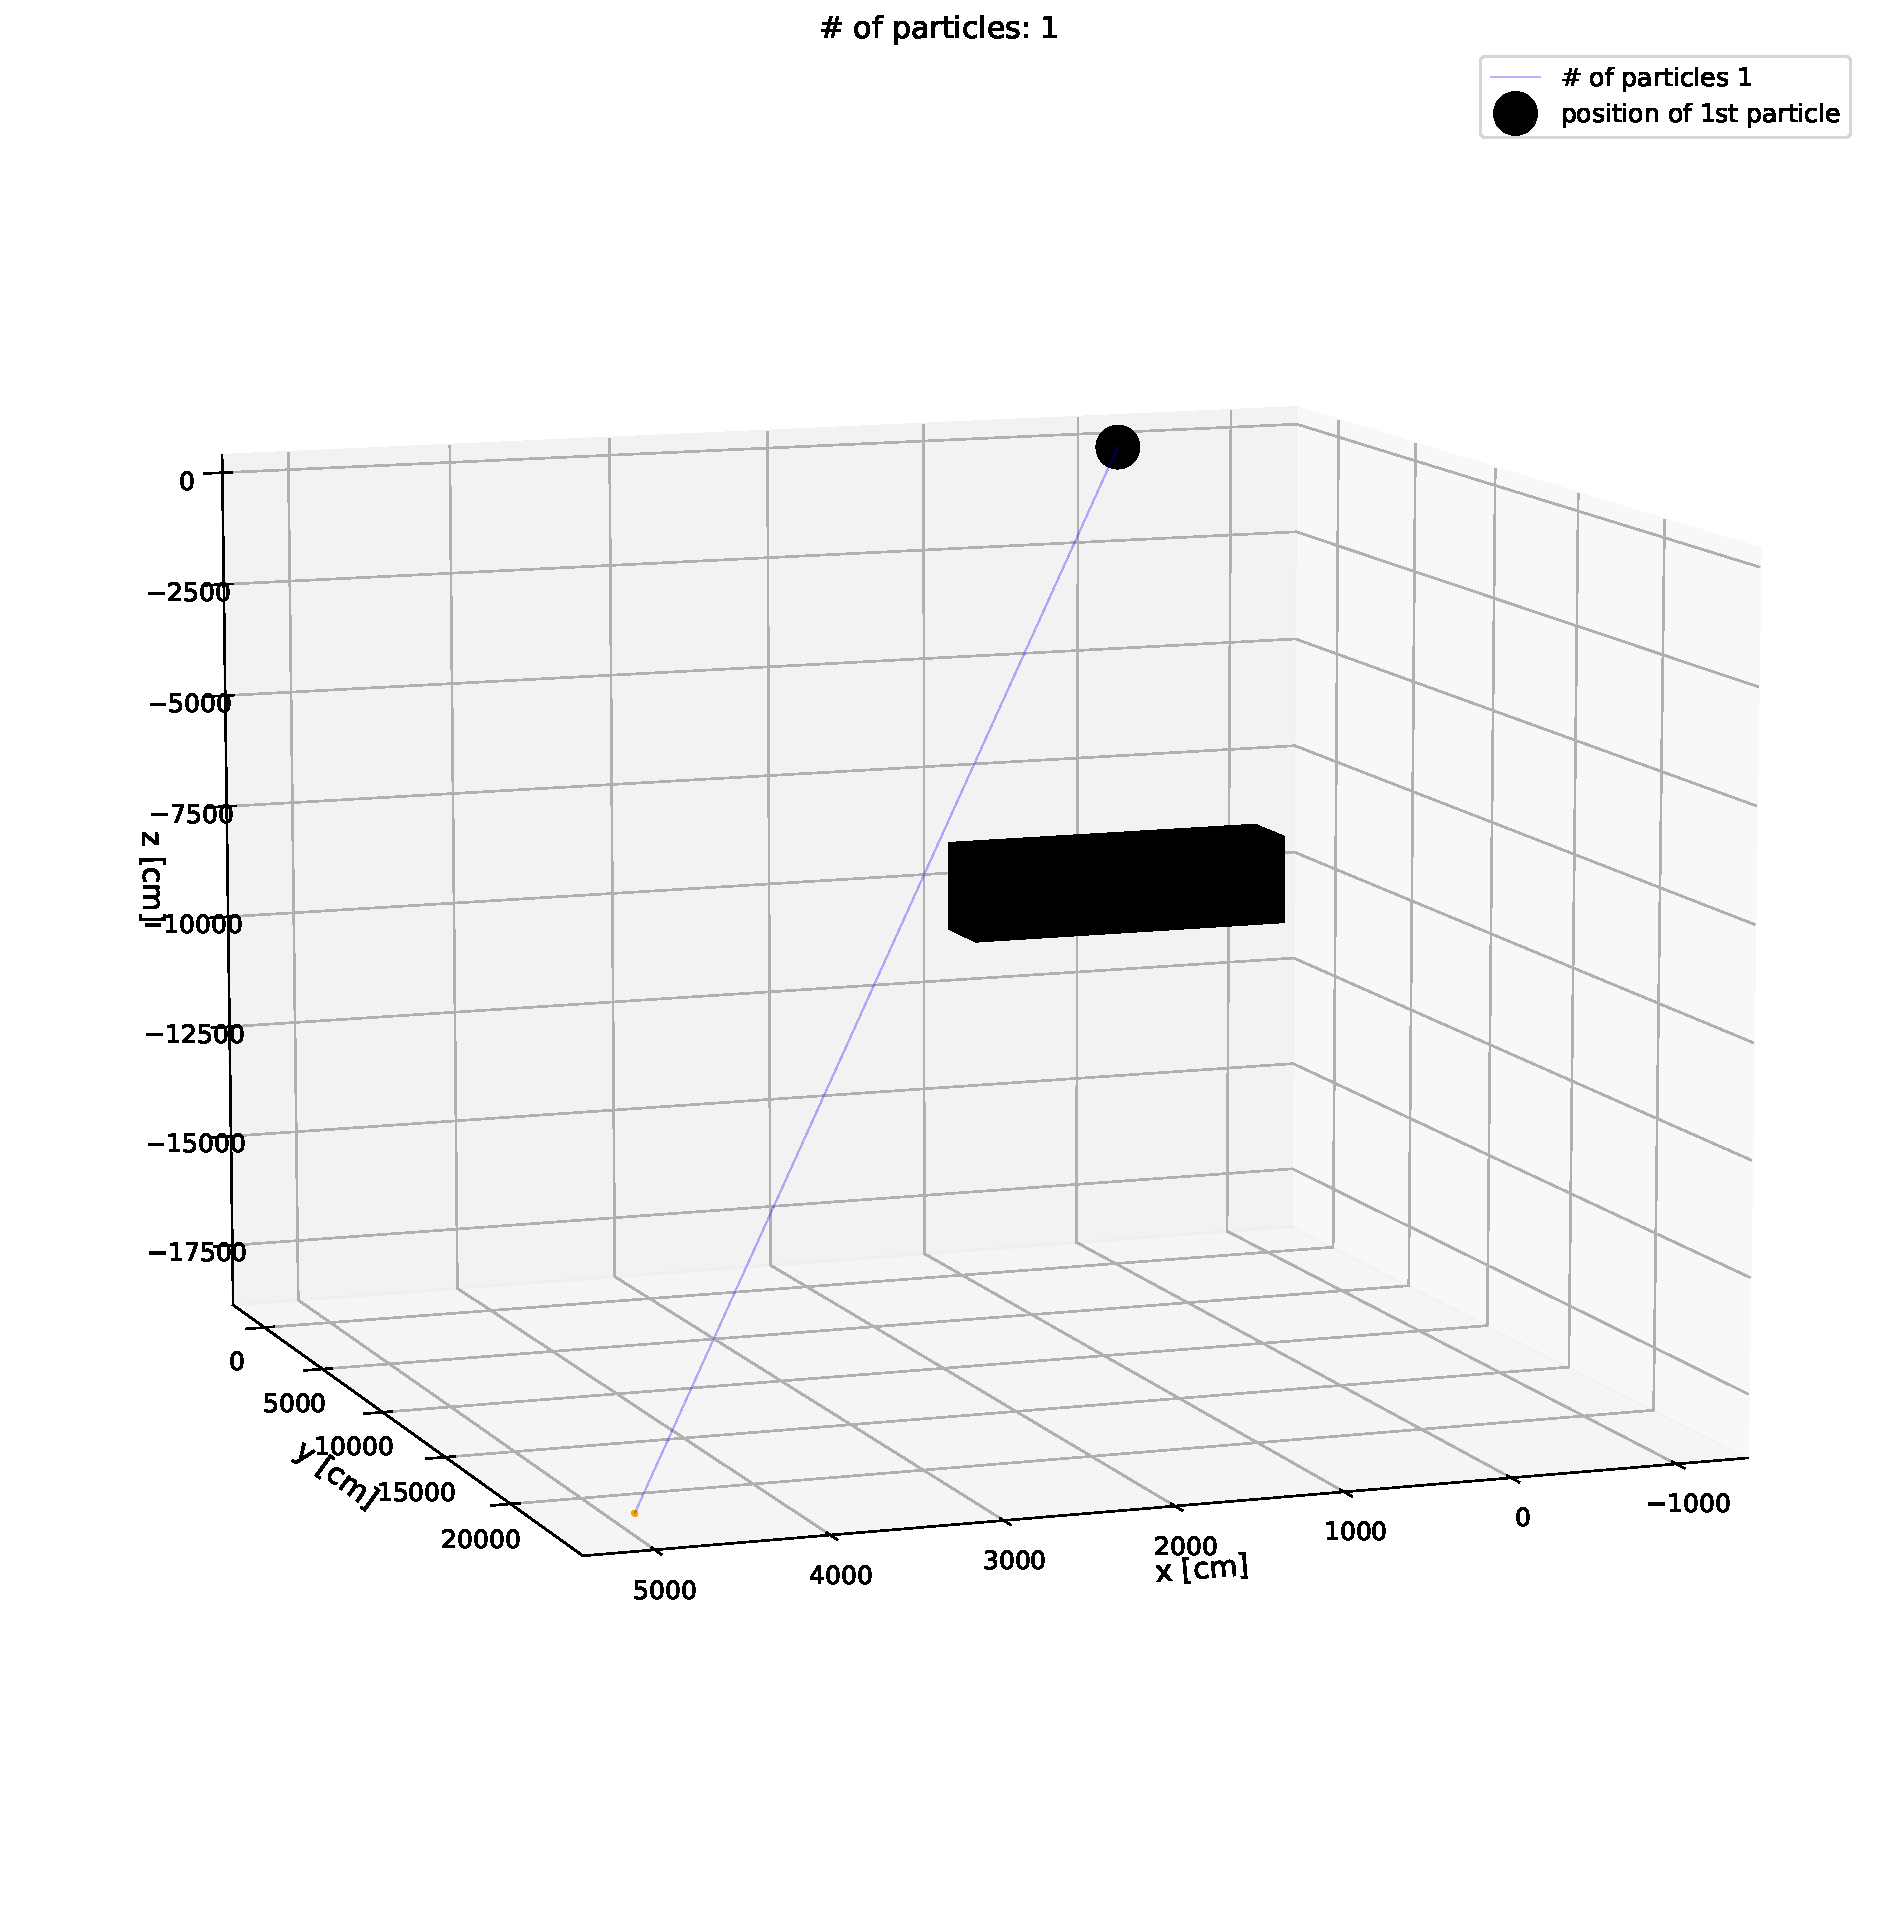
\includegraphics[width=0.7\textwidth]{plot_3D_start_end.pdf}
    \caption{Veranschaulichung der Start und Endpunkte der Myonen die den Detektor erreicht haben.
    Die Punkte werden durch eine blaue gerade Linie verbunden. 
    Alle Myonen werden bei \SI[]{1259}[]{m} gestoppt.}
    \label{fig:3d-plot}
\end{figure}
\section{Simulation der Myonen mit PROPOSAL}

PROPOSAL propagiert die Teilchen, hat allerdings gegenüber der echten Welt Einschränkungen.
Durch die Energieschnitte (siehe Kap. \ref{sec:pp-theorie}) wird ein Teil immer
kontinuierlich genähert. Durch die Wahl eines kleinen $v_\mathrm{cut}$ ist dieser Effekt 
allerdings vernachlässigbar.
Des Weiteren muss bezüglich der Messunsicherheit PROPOSALs 
bedacht sein, dass sich PROPOSAL nicht in allen Energiebereichen 
und Szenarien vergleichen kann mit echten Daten, sondern dort sich mit
ähnlichen Simulationsprogrammen vergleicht. 


\section{Ergebnisse}
% \section{Konfiguration von PROPOSAL}
\label{sec:pp-config}

Die Ergebnisse der Simulation sind in Tabelle \ref{tab:wassertiefen_tabelle} aufgelistet.
Auf den Detektor umgerechneten Detektorzählraten sind in \ref{fig:results} dargestellt.
In Abb. \ref{fig:pp_energiespekten} ist das Energiespektrum der ursprünglichen Myonen 
dieser die am Detektor angekommen sind, sowie die Endenergien am Detektor. 

Es ist ein klarer Zusammenhang zwischen Wassertiefe und Myonenanzahal bzw. Detektorrate erkennbar.
Damit ist bestätigt, sich Wassertiefen in alten Berbauregionen mithilfe der Myographie messen lassen.
% Es ist in Abb. \ref{} und \ref{} jeweils das Energiespektrum der Myonen am Detektor sowie
% deren ursprüngliches zu sehen. 
Zwischen der höchsten (\SI[]{840}[]{m}) und niedrigsten (\SI[]{0}[]{m}) Wasserhöhe
besteht in der Detektorrate ein Unterschied von
\begin{equation}
    \Delta\Phi = \SI[]{33.2 e - 3}[]{\frac{\mathrm{Myonen}}{\mathrm{Tag}}}
    \quad \mathrm{oder}\quad \SI[]{13,06}{\%}.
\end{equation}
Zwischen den extremsten Wasserschichten Schichten sinkt also die Rate um.
Pro \SI[]{100}[]{m} sind das im Mittel eine Reduktion von
\begin{align}
    \SI[]{4.0 e-3}[]{\frac{\mathrm{Myonen}}{\mathrm{Tag}}} \quad \mathrm{oder}\quad  \SI[]{1,55}[]{\%}
\end{align}
Wird nun die wesentlich dichtere Dolomit Schicht zwischen \SI[]{748}{m} und \SI[]{840}[]{m}
betrachtet wird im Kontrast zu der darunter liegenden Tonsteinschicht
, keine signifikante Änderung der Abschwächungen der Raten beobachtet.
Es ist außerdem festzustellen, dass die Dichten der Schichten 
wenig Einfluss haben auf die Änderung der Absorption bei fixen Hohlraumvolumen. 

\begin{table}[h]
    \caption{Für verschiedene Wassertiefen, die Anzahl an detektierten Myonen
     sowie deren prozentuales Verhältnis $N_\mathrm{d}/N_0$ zur Gesamtmenge an propagierten Myonen.}
    \centering\begin{tabular}{c c c}
        Wassertiefe / \si[]{m} & \# Teilchen &  \% $N_\mathrm{d}/N_0$ \\
        0   & \num{2344409} & \num{23.44} \\
        100 & \num{2303835} & \num{23.04} \\
        200 & \num{2266474} & \num{22.66} \\
        300 & \num{2227742} & \num{22.28} \\
        324 & \num{2218556} & \num{22.19} \\
        400 & \num{2192224} & \num{21.92} \\
        500 & \num{2155066} & \num{21.55} \\
        600 & \num{2118887} & \num{21.19} \\
        700 & \num{2085579} & \num{20.86} \\
        748 & \num{2070024} & \num{20.70} \\
        800 & \num{2051255} & \num{20.51} \\
        840 & \num{2038287} & \num{20.38} \\
    \end{tabular}
    \label{tab:wassertiefen_tabelle}
\end{table}

\begin{figure}[]
    \centering
    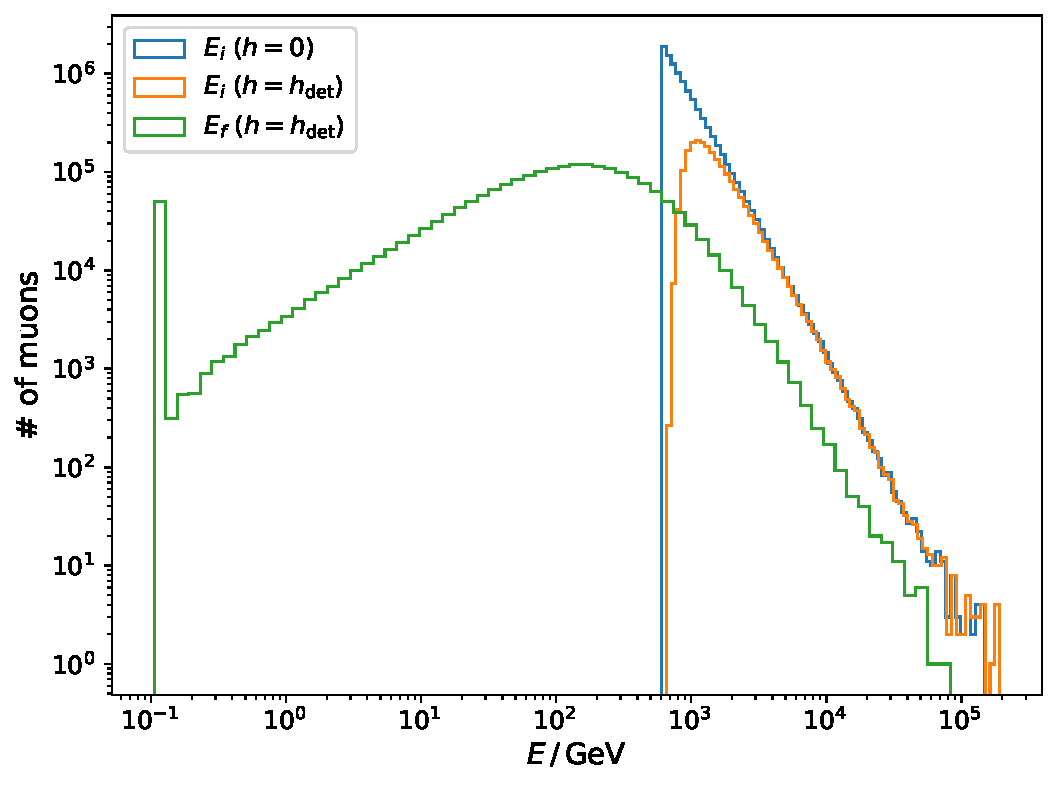
\includegraphics[width=0.8\textwidth]{EcoMug_gaisser_30deg_1e7_min6e2_max2e5.hdf_v=1.pdf}
    \caption{Das Energiespektrum für eine Wassertiefe von \SI[]{800}[]{m}.
        In Blau die ursprünglichen Myonen auf der Erdoberfläche.
        In Orange diejenigen, die angekommen sind. 
        In Grün die Endenergie der Myonen am Detektor.}
    \label{fig:pp_energiespekten}
\end{figure}


\begin{figure}[h]
    \centering
    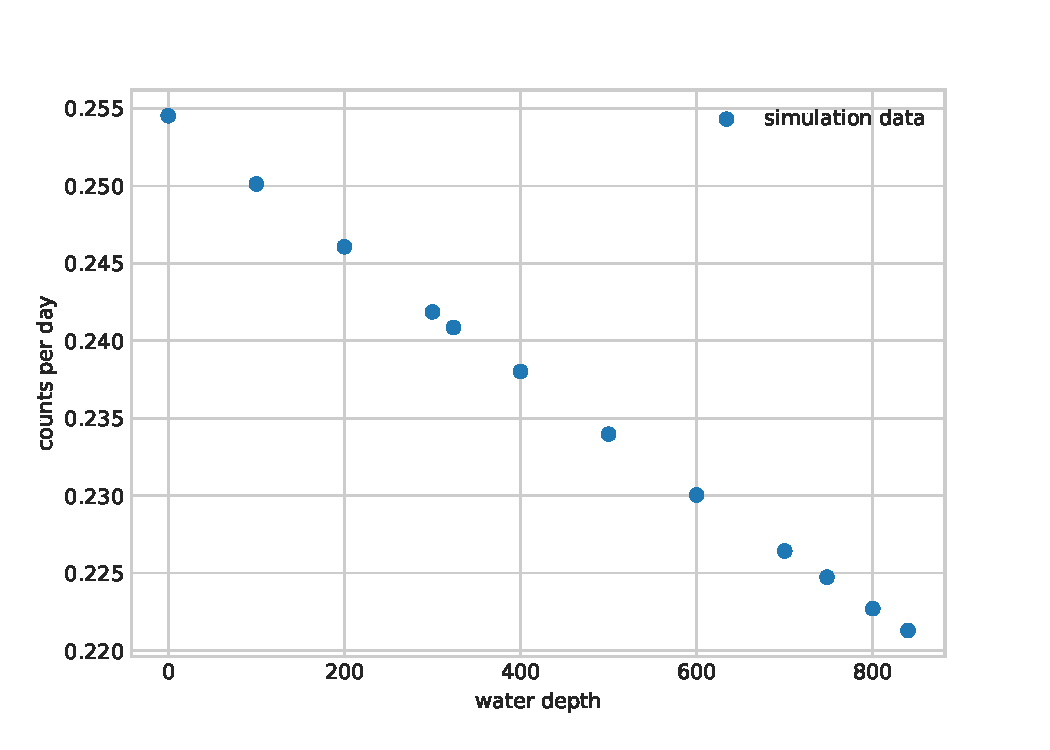
\includegraphics[width=0.8\textwidth]{results_plot.pdf}
    \caption{Detektorraten in Teilchen pro Tag gegen die 
    Wasser Tiefe.}
    \label{fig:results}
\end{figure}